\documentclass[a4paper,12pt]{article} %Dokumendiklassi defineerimine ja väljastatava teksti suuruse seadistamine       
\usepackage{graphicx} %Võimaldab teksti sees kasutada jooniseid
\usepackage[top=2.5cm, bottom=2.5cm, left=3cm, right=3cm]{geometry} %Määrab ära lehekülje suuruse
\usepackage{titlesec} %Vajalik pealkirjade modifitseerimiseks
\usepackage{longtable} %Vajalik pakett, et saaks teha üle ühe leheküljelisi tabeleid
\usepackage{multirow} %Vajalik, kui tahta tabelites mitut rida kokku panna
\usepackage{todonotes} %Vajalik, kui tahta lisada töösse todo märkmeid
\usepackage{url} %Vajalik, kui töös on kasutusel URL aadress. Sel juhul märkida URL tagi vahele ning LaTeX ei hakka seda lahti kompileerima eraldi käskudeks vms
\usepackage[figure,table,page,section]{totalcount} %Jooniste, tabelite, lehtede ja peatükkide arv
\usepackage{float} %Vajalik töös olevate tabelite ja jooniste vormistamiseks
\usepackage{blindtext}
\usepackage{scrextend}
\addtokomafont{labelinglabel}{\sffamily}
\usepackage{longtable} %Korda tabeli päist uuel lehel
\usepackage{color,xcolor,colortbl}% Värvid
\definecolor{codegreen}{rgb}{0,0.6,0}
\definecolor{codegray}{rgb}{0.5,0.5,0.5}
\definecolor{codepurple}{rgb}{0.58,0,0.82}
\definecolor{rowgray}{gray}{0.85}
\usepackage{listings} %Koodi värvimiseks
\lstset{
    breaklines=true,
    frame=single
  }
\lstnewenvironment{SQL}
  {\lstset{
    breaklines=true,
    language=SQL,
    frame=single,
    framesep=5pt,
    basicstyle=\normalsize,
    %basicstyle=\footnotesize,
    commentstyle=\color{codegreen},
    keywordstyle=\color{blue},
    numberstyle=\tiny\color{codegray},
    stringstyle=\color{codepurple},
    keepspaces=true,                 
    numbers=left,                    
    numbersep=2pt,                  
    showspaces=false,                
    showstringspaces=false,
    showtabs=false,                  
    tabsize=2
  }}
  {}

\usepackage[estonian]{babel} %Eestikeelsete tähtede kasutamise võimalus
\usepackage[T1]{fontenc} %Vajalik vene ja eesti  keelsete tähtede kasutamiseks
\usepackage[utf8]{inputenc} %UTF8 dekodeerimise kasutamine

\addto\captionsestonian{\def\refname{\centerline{Kasutatud kirjandus}}} %Muudab viidete nime kasutatud kirjanduseks ning paigutab lehe keskele
\addto\captionsestonian{\def\listfigurename{\centerline{Jooniste loetelu}}} %Muudab jooniste nimekirja nime jooniste loeteluks ning paigutab selle lehe keskele
\addto\captionsestonian{\def\listtablename{\centerline{Tabelite loetelu}}} %Muudab tabelite nimekirja nime tabelite loeteluks ning paigutab selle lehe keskele
\addto\captionsestonian{\def\contentsname{\centerline{Sisukord}}}
	
\usepackage{tocloft} %Selleks, et modifitseerida sisukorda
\usepackage{amssymb} %Erisümbolid
\renewcommand{\labelitemi}{\tiny$\blacksquare$} %Loetelude ees kuvatakse ruudukesi

\usepackage{caption} %Vajalik tabelite ja jooniste pealkirjastamisel
\captionsetup{labelsep=period} %Lisab tabeli või joonise nime lõppu punkti

\usepackage{verbatimbox} %Koodi kuvamine lehe keskel

\titlelabel{\thetitle.\quad} %Lisab pealkirjade lõppu punkti

\usepackage{times} %Tekst on Times tüüpi
\usepackage{fancyhdr} %Võimaldab kasutada päiseid ja jaluseid
\setlength{\parindent}{0cm} %Lõigu taane on seatud nulliks
\usepackage{setspace} %Vajalik teksti vahede seadistamiseks
\onehalfspacing %Ridade vahel on 1,5 tähe kõrgusest
\setlength{\parskip}{12pt}%Lõiguvahe

\usepackage{hyperref} %Muudab lingid klikitavaks

\hyphenation{} %Ebakorrektse poolitamise parandamine kujul: \hyphenation{üliõpilas-kood lehe-küljed}

\titleformat{\section}{\normalfont\Large\bfseries}{\thesection}{16pt}{} %Sectioni tekstisuurus
\titleformat{\subsection}{\normalfont\large\bfseries}{\thesubsection}{14pt}{} %Subsectioni tekstisuurus
\titleformat{\subsubsection}{\normalfont\normalsize\bfseries}{\thesubsubsection}{12pt}{} %Subsubsectioni tekstisuurus

%\titlespacing*{\section}{0pt}{44pt}{18pt} %Sectioni ees, ülal ja all olev ruum
\titlespacing*{\subsection}{0pt}{24pt}{12pt} %Subsectioni  ees, ülal ja all olev ruum
\titlespacing*{\subsubsection}{0pt}{12pt}{12pt} %Subsubsectioni ees, ülal ja all olev ruum

\newcommand{\sectionbreak}{\clearpage} % Iga section algab uuelt lehelt

\begin{document}

%------------------------------TIITELLEHT---------------------------------
\thispagestyle{fancy} %Leht sisaldab päist ja jalust
\renewcommand{\headrulewidth}{0pt} %Eemaldab päisest horisontaalse joone
\renewcommand{\footrulewidth}{0pt} %Eemaldab jalusest horisontaalse joone
\headheight = 60pt %Paneb paika päise laiuse (vastavalt kompilaatori soovitusele)
\footskip = 9pt %Jaluse ruum
\headsep = 0pt %Vähendab päise ja teksti vahelise kauguse nullini

\chead{ %Paigutab järgneva teksti päises keskele
 \textsc{\begin{Large} %Tekst suurtähtedega ja suuremaks
	tallinna tehnikaülikool\\
	\end{Large} }
	Infotehnoloogia teaduskond\\
	Informaatika instituut\\
	Infosüsteemide õppetool
}
\vspace*{140pt} %Tekitab lehe alguse ja teksti vahele tühja ala vastava laiusega

\begin{center} %Tekst keskele
\begin{LARGE}
PostgreSQL-i põhise meta-andmetega juhitavate veebirakenduste kiirprogrammeerimiskeskkonna projekteerimine ja realiseerimine\\[20pt]
\end{LARGE}
Magistritöö\\[60pt]
\end{center}

\begin{flushright} %Joondab teksti paremale
\begin{tabular}{p{80pt}p{100pt}}
Üliõpilane:&Rait Raidma\\
Üliõpilaskood:&143682IAPM\\
Juhendaja:&dotsent Erki Eessaar\\
\end{tabular}
\end{flushright}

\cfoot{Tallinn\\2016} %Lisab asukoha ja kuupäeva jalusesse
\pagebreak %Lehe lõpp

%---------------------------AUTORIDEKLARATSIOON-------------------------
\section*{\begin{center}
 Autorideklaratsioon
\end{center}}

Kinnitan, et olen koostanud antud lõputöö iseseisvalt  ning seda ei ole kellegi teise poolt varem kaitsmisele esitatud. Kõik töö koostamisel kasutatud teiste autorite tööd, olulised seisukohad, kirjandusallikatest ja mujalt pärinevad andmed on töös viidatud.\\[50pt]

\begin{center}
\begin{tabular}{cc}
......................................................&......................................................\\
\textit{(kuupäev)}&\textit{(allkiri)}\\
\end{tabular}
\end{center}

\pagebreak

%---------------------------ANNOTATSIOON---------------------------------
\section*{\begin{center}
Annotatsioon
\end{center}}

Lõputöö on kirjutatud eesti keeles ning sisaldab teksti \totalpages{} leheküljel, \totalsections{} peatükki, \totalfigures{} joonist, \totaltables{} tabelit.
\pagebreak
%-----------------------------ABSTRACT-----------------------------------
\section*{\begin{center}
Abstract
\end{center}}
The thesis is in estonian and contains \totalpages{} pages of text, \totalsections{} chapters, \totalfigures{} figures, \totaltables{} tables.
\pagebreak
%---------------------LÜHENDITE JA MÕISTETE SÕNASTIK---------------------
\section*{\begin{center}
Lühendite ja mõistete sõnastik
\end{center}}
\begin{tabular}{p{4cm}p{10cm}} %Tabel, mille esimese lahtri laius on 4cm.
SQL&\textit{Structured Query Language}, struktureeritud andmebaasikeel andmete käitlemiseks, õiguste jagamiseks ning andmebaasiobjektide haldamiseks\\
FSF&\textit{Free Software Foundation}, MTÜ, mis propageerib arvuti kasutajate vabadust ja kaitseb vaba tarkvara kasutajate õigusi\\
OSI&\textit{Open Source Initiative}, Organisatsioon, mis propageerib avatud lähtekoodiga tarkvara\\
Juurutama&\textit{Deploy}, Tarkvara või riistvara töölepanekuga seotud protsesside - installeerimine, konfigureerimine, käitamine, testimine - läbimine \cite{Vallaste}\\
CRUD&\textit{Create Read Update Delete}, Lühend, mis tähistab andmetega manipuleerimise nelja põhitegevust: loomine, lugemine, muutmine ja kustutamine\\
Meta-andmed&Andmed andmete kohta\\
Meta-andmetega juhitav&Süsteemi käitumist ja väljanägemist juhitakse andmetega.\\
URL&\textit{Uniform Resource Locator}, Internatiaadress. Viit arvutivõrgus olevale ressursile. \cite{Vallaste}\\
Kiirprogrammeerimine&\textit{Rapid Application Development}, Arendussüsteem, mis annab programmeerijatele võimaluse kiiresti programme koostada. Üldiselt on RAD-süsteemides rida graafiliste kasutajaliideste loomiseks mõeldud tööriistu, mis oluliselt lühendab taoliste liideste loomisele kuluvat aega \cite{Vallaste}\\
DOM&\textit{Document Object Model}, dokumendiobjektide mudel. Eeskiri selle kohta, kuidas objekte (tekst, pildid, pealkirjad, lingid jne.) veebilehel esitada. DOM määrab ära, millised atribuudid kuuluvad millise objekti juurde ning kuidas objekte ja atribuute käsitleda \cite{Vallaste}\\
HTML&\textit{HyperText Markup Language}, hüpertekst-märgistuskeel. Enimlevinud kodeerimissüsteem (tekstivorming) veebidokumentide loomiseks. HTML koodid ehk märgendid määravad ära selle, kuidas veebileht arvutiekraanil välja näeb \cite{Vallaste}\\
CSS&\textit{Cascading Style Sheets}, kaskaadlaadistik. Veebilehtede valmistajatele ja kasutajatele mõeldud laadistik. Laadilehed (style sheets) kirjeldavad, kuidas HTML dokumente esitada kuvaril, printeril või kõnesüntesaatorist kostva kõnena \cite{Vallaste}\\
\end{tabular}
\pagebreak
%----------------------------SISUKORD----------------------------------
\tableofcontents
\newpage
%----------------------JOONISTE NIMEKIRI-------------------------------
\listoffigures
\pagebreak
%----------------------TABELITE NIMEKIRI---------------------------------
\listoftables
\pagebreak
%-----------------------------SISSEJUHATUS------------------------------- 
\section{Sissejuhatus}
\label{Sissejuhatus} %Võimaldab pealkirjale viidata \ref käsuga
Järgnevalt on välja toodud, miks ning kuidas antud tööd tehakse.

\subsection{Taust ja probleem}
Töö idee sai alguse TTÜ-s õpetatavast ainest ``Andmebaasid II'', mille raames tuleb üliõpilastel ühe õpiväljundina luua andmebaas koos seda kasutava rakendusega, kus rakendus suhtleb andmebaasiga läbi andmebaasiliidese. Antud aines võib kasutada andmebaasisüsteeme PostgreSQL \cite{PostgreSQL} ja Oracle \cite{Oracle_DB}. Juhul, kui andmebaas on loodud Oracle andmebaasisüsteemi abil, siis on üliõpilastel rakenduse loomiseks võimalus kasutada kiirprogrammeerimiskeskkonda Oracle APEX \cite{Oracle_APEX}. PostgreSQL andmabaasisüsteemiga loodud andmebaasi korral tuleb rakendus programmeerida kasutades PHP-d \cite{PHP}. See tähendab, et üliõpilane ei saa keskenduda täielikult andmebaasi täiustamisele vaid peab tegelema ka lisaprogrammeerimisega. Töö tulemusena valmiva süsteemi abil peaks üliõpilastel olema lihtsam luua näidisrakendusi, mis kasutavad andmebaasisüsteemina PostgreSQL-i. Samas leiab autor, et valmiv süsteem on piisavalt võimekas, et leida raakendust teisteski kohtades.\par
Töö valmis 2016. aasta kevadel Tallinna Tehnikaülikoolis.

\subsection{Ülesande püstitus}
Töö eesmärgiks on disainida ning realiseerida PostgreSQL põhine kiirprogrammeerimiskeskkond, mille abil saaks luua teisi veebipõhiseid rakendusi, mis hoiavad andmeid samas andmebaasiserveris kui loodav süsteem. Loodavates rakendustes peab andmete pärimine, lisamine, muutmine ning kustutamine käima läbi andmebaasiliidese. Kogu vajalik info rakenduste kuvamiseks ja käitumise juhtimiseks tuleb hoida loodava süsteemi meta-andmete andmebaasis.\par
Loodav süsteem peab toetama PostgreSQL 9.4 ja PHP 5.5.0 ning tuleb välja anda vabavara litsentsi all, et soodustada süsteemi laialdasemat levikut.

\subsection{Metoodika}
Esiteks tuleb uurida, kas liideste kasutamine andmebaasi poole peal annab süsteemile mingi eelise. Seejärel tuleb selgeks teha, kas ja kuidas saab ühest andmebaasist suhelda teiste andmebaasidega, mis asuvad samas andmabaasiserveris. Ning viimasena, kuidas küsida teistest andmebaasidest infot liideste kohta.
Lisaks uurin, milliseid sarnaseid süsteeme on veel olemas ning kuidas need on üles ehitatud.\par
Töö tulemusena valmib süsteem, mille abil saab luua veebipõhiseid rakendusi, mis kasutavad andmebaasiga suhtlemiseks andmebaasiliideseid. Töö tulemuse valideerimiseks loodakse näidisrakendus, kus realiseeritakse õppejõu poolt ette antud kasutusjuhud, mis sarnanevad üliõpilastöödes esinevatele kasutusjuhtudele.
\subsection{Ülevaade tööst}
TODO
\pagebreak

\section{Teoreetiline taust}
Järgnevalt viiakse lugeja kurssi vajalike teadmistega, mida on vaja süsteemi loomiseks.

\subsection{Andmebaasi avalik liides}
\label{andmebaasi_avalik_liides}
Liides on sõltumatute süsteemide vaheline leping, kus on kirjeldatud, millisel viisil saab üks süsteem teisega suhelda.
Andmebaasis saab liideseid kirjeldada rutiinidena ja vaadetena (vt Joonis \ref{fig_andmebaasi_avalik_liides}).

\begin{figure}[H]
\begin{center}
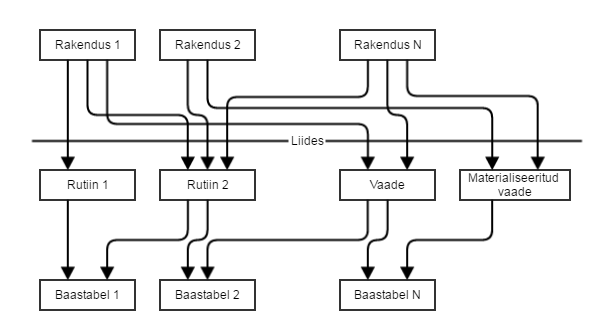
\includegraphics[bb=0 0 606 330,scale=0.6]{./diagrams/db-interface.png}
\caption{Andmebaasi avalik liides}
\label{fig_andmebaasi_avalik_liides}
\end{center}
\end{figure}

\subsubsection{Vaadete kasutamise eelised ja võimalused}
\begin{itemize}
\item Võimaldavad igale rakendusele saab luua spetsiifilise vaate andmetest, ilma et oleks vaja teha muudatusi andmemudelis.
\item Võimaldavad vähendada rakenduse koodi ja andmemudeli vahelist sidusust.
See võimaldab teha muudatusi andmemudelis, ilma et olemasolev rakendus katki läheks.
\item Neile saab anda rakenduse-spetsiifilised veerunimed, andmetüübid ja pikkused, mis võimaldab otse andmete sidumist rakenduses kasutatavate mudelitega.
\item Võimaldavad jõustada andmete turvamist. Erinevatele kasutajagruppidele saab kuvada andmeid erineval kujul, nii et kasutaja näeb üksnes neid andmeid, mida ta on volitatud nägema. PostgreSQL andmebaasisüsteemis tuleks lisaks kasutada turvabarjääri \textit{WITH (security\_barrier)} lisatingimust. See takistab peidetud ridade kuvamist ka juhul, kui kasutatakse kuritahtlikult valitud funktsioone ja operaatoreid, et näha varjatud infot \cite{PostgreSQLRulesAndPrivileges}
\item Võimaldavad pärida andmeid erinevatest tabelitest ja andmebaasidest, peites kasutajate eest päringu tegeliku keerukuse. Vaate koostamiseks vajalik päring on eelnevalt kompilleeritud ja optimiseeritud, et tagada parem jõudlus. Vaated kasutavad päringu täitmisel baastabelitele loodud indekseid.
\item Võimaldavad varjata rakenduse eest baastabelites olevaid disaini -ja andmevigasid, andes lisaaega nende parandamiseks.
\item Võimaldavad kuvada samu andmeid erineval kujul ühendatuna, kasvõi nt XML-na või JSON-na.
\item Läbi vaadete, mis vastavad teatud tingimustele, on võimalik teha andmemuudatusi baastabelites, kui realiseerida INSTEAD OF triggerid.
\end{itemize}
\cite[lk 172-173]{BuildingTheAgileDatabase}

\subsubsection{Vaadete kasutamisel tekkida võivad probleemid PostgreSQL andmebaasisüsteemi korral}
\begin{itemize}
\item Andmebaasisüsteem ei suuda kasutada põhipäringu tingimust (\textit{WHERE} klausel) vaate alampäringus kui vaate alampäringus tehakse ühendi leidmist \textit{UNION} või \textit{UNION ALL} või kui alampäring sisaldab aknafunktsiooni (nt \textit{ROWNUMBER() OVER()} ja \textit{LAG() OVER()})
\item Kui vaate alampäring sisaldab agregaatfunktsiooni (ilma \textit{GROUP BY} klauslita), \textit{ROWNUM} pseudoveergu, aknafunktsiooni \textit{ROWNUMBER() OVER()} või rekursiivset päringut, siis täidetakse vaate põhjal tehtud päring ja vaate alampäring eraldi.
\item Vaate turvabarjääri \textit{WITH (security\_barrier)} kasutamine seab piirangud vaate tingimusklauslite ning vaate põhjal tehtud päringu tingimusklauslite mestimisele, mille tulemusena loodav täitmisplaan ei pruugi olla optimaalne
\item Kui vaate alampäringus viidatakse teistele vaadetele, siis nende vaadete alampäringud täidetakse eraldi, mille tulemusena suureneb päringu täitmiskiirus.
\end{itemize}
\cite[lk 101-102]{VaadeteMojuParingutele}

\subsubsection{Rutiinide kasutamise eelised}
\begin{itemize}
\item Üle võrgu saadetavate andmete ja SQL koodi hulk hoitakse minimaalsena, mille tulemusel suureneb rakenduse jõudlus.
\item Rutiinide kood on andmebaasi serveris eelnevalt kompilleeritud ja optimiseeritud, suurendades rutiini täitmise efektiivsust.
\item Andmetöötluse jaoks kasutatakse andmebaasiserveri jõudlust, mitte rakendusserveri ega kliendi masina oma.
\item Rutiinis olevat SQL koodi on lihtsam testida ja optimiseerida, kui rakendusse sisse kirjutatud SQL-i.
\item Rutiinide käivitusõiguste abil saab piirata ligipääsu teatud rollidele ning suurendada seeläbi turvalisust.
\item Rutiinis käivitatavad laused tehakse ühe transaktsiooni jooksul. See aitab vältida osalisi andmemuudatusi, kus üks osa muudatustest läks läbi, teine osa aga mitte.
\end{itemize}
\cite[lk 179, 195]{BuildingTheAgileDatabase}

\subsubsection{Rutiinide puudused}
\begin{itemize}
\item Koodifunktsionaalsus on piiratud.
\item Keerulisemaid rutiine ei pruugi olla võimalik teisaldada ühelt andmebaasisüsteemilt teisele.
\item Rutiine on keerulisem kapseldada ning selle tulemusena võib üks ärireegel olla jaotatud mitme rutiini vahele, mis teeb ärireegli haldamise keerulisemaks.
\end{itemize}
\cite{StoredProcProsAndCons}

\subsubsection{Järeldus andmebaasiliideste kasutamise kohta}
Andmebaasiliidesed annavad kasutajale võimaluse viia andmebaasi ja rakenduse vaheline sidusus minimaalseks ning suurendada andmete turvalisust ja terviklikust. Mõningatel juhtudel võivad aga vaated mõjuda jõudlusele nagatiivselt ning rutiinides võib mõningate tegevuste täitmiseks loodava koodi kirjutamine olla keerulisem kui rakenduse kihis. Autori arvates ei kaalu negatiivsed aspektid üle positiivseid ning seetõttu leiab autor, et andmebaasiliideseid tuleks võimaluse korral kasutada.

\subsection{Ühendumine teiste andmebaasidega}
Kui loodav süsteem installida serverisse, kus on mitu andmebaasi, siis  peab kõikide nende andmebaaside põhjal olema võimalik luua rakendusi. Selleks peab loodav süsteem olema võimeline tegema päringuid samas andmebaasiserveris olevatesse andmebaasidesse. PostgreSQL andmebaasisüsteemis pole realiseeritud andmebaaside vahelisi viitasid ning seetõttu ei saa koostada päringuid kujul:
\begin{SQL}
select * from other_db_name.schema_name.table_name;
\end{SQL}
Eelnev päring annab tulemuseks veateate:
\begin{lstlisting}
ERROR:  cross-database references are not implemented: "other_db_name.schema_name.table_name"
\end{lstlisting}
Selleks, et ühenduda väliste PostgreSQL andmebaasidega, tuleb kasutada kas dblink või postgres\_fdw moodulit.

\subsubsection{dblink}
\label{dblink}
Mooduli installeerimine:
\begin{SQL}
CREATE EXTENSION IF NOT EXISTS dblink;
\end{SQL}
Andmete küsimiseks välisest andmebaasist tuleb ette anda andmebaasi nimi, kasutaja ja parool ning lause, mida käivitada soovitakse. Päring käivitatakse välises andmebaasis. Päringuks võib olla iga SQL lause, mis tagastab read.\cite{PostgreSQLdblink} Allpool on toodud näide päringu koostamisest dblink mooduli abil.
\begin{SQL}
SELECT schema_name, owner_id
FROM dblink(
  'dbname=external_database_name user=external_database_user password=external_database_user_password',
  'SELECT upper(nspname), nspowner FROM pg_catalog.pg_namespace;'
) AS (
  schema_name varchar,
  owner_id int
);
\end{SQL}

\subsubsection{postgres\_fdw}
Selle mooduli poolt pakutav funktsionaalsus kattub suurel määral \textit{dblink} \ref{dblink} mooduli funktsionaalsusega, kuid pakub standardsemat süntaksit päringute koostamiseks ning võib \textit{dblink}-i kohati edestada jõudluse poolest.\par
\textit{postgres\_fdw} loob ühenduse välise serveriga siis, kui tehakse esimene päring välise tabeli vastu. Seda ühendust hoitakse alles ning kasutatakse järgmiste päringute jaoks sama sessiooni piires. Kui väliselt serverilt küsitakse infot erinevate kasutajatena \textit{user mappings}, siis luuakse iga kasutaja jaoks uus ühendus.\par
\textit{postgres\_fdw} üritab optimeerida väliseid päringuid, et vähendada küsitavate andmete hulka. Selleks saadetakse koos päringuga \textit{WHERE}-tingimus ning ei laeta alla veerge, mida pole päringu täitmiseks vaja. Selleks et vältida valesid päringutulemusi, ei saadeta \textit{WHERE}-tingimusi, kui kasutatakse midagi peale sisse ehitatud andmetüüpide, operaatorite ja funktsioonide või kui operaatorid ja funktsioonid pole muutumatud (\textit{immutable}). \cite{PostgreSQLfdw}\par
\textit{postgres\_fdw} võimaldab lisaks andmete küsimisele (\textit{SELECT}) ka andmeid lisada (\textit{INSERT}), muuta (\textit{UPDATE}) ja kustutada (\textit{DELETE}) välisest tabelist. Küll aga ei võimalda antud moodul välja kutsuda välises andmebaasis olevaid funktsioone kujul:
\begin{SQL}
SELECT function_from_external_database();
\end{SQL}

\subsubsection{Mooduli valik}
Kuna loodav süsteem peab suutma välja kutsuda välistes andmebaasides olevaid funktsioone, siis pole tuleb kasutada \textit{dblink} \ref{dblink} moodulit.

\subsection{Andmebaasiobjektide kirjelduste küsimine}
\label{andmebaasi_objektide_kirjelduste_küsimine}
Loodav süsteem peab teistest andmebaasidest küsima infot andmebaasibjektide kohta, et kuvada süsteemi kasutajale info andmebaasiliidestest, mida rakenduse loomisel on võimalik kasutada. Selleks vajaliku info saab küsida süsteemikataloogidest: information\_schema ja pg\_catalog.
Information\_schema sisaldab vaateid andmebaasis olevate objektide kohta. Kuna information\_schema on defineeritud SQL standardis, siis võib eeldada, et selle formaat ei muutu ning seetõttu tuleks eelistada seda kataloogi, et vältida loodava rakenduse katki minekut  järgmiste PostgreSQL versioonide korral. \cite{PostgreSQLInformationSchema} Küll aga ei sisalda information\_schema infot PostgreSQL-spetsiifiliste võimaluste kohta. Selleks tuleb pöörduda pg\_catalog-i poole. Pg\_catalog-st saab lisaks pärida infot samasse andmebaasiserverisse kuuluvate andmebaaside, materialiseeritud vaadete ning kasutajate paroolide kohta. \cite{PostgreSQLSystemCatalogs} Täpsem loetelu olulisematest süsteemikataloogide vaadetest, mida süsteemi loomisel vaja läheb, on välja toodud Lisa 1-es.

\subsection{Eksisteerivate programmide analüüs}
Töö käigus uuriti, milliseid sarnaseid süsteeme on veel loodud ning kuidas need on üles ehitatud. Järgnevalt on esitatud ülevaade nendest süsteemidest.
\subsubsection{Oracle Application Express (APEX)}
Oracle APEX on veebipõhine rakendus loomaks kiirelt ja lihtsalt teisi veebipõhiseid rakendusi. Kogu süsteem on juhitav andmebaasis hoitavate metaandmetega. APEX kasutab tööks Oracle anembaasisüsteemi.\par
APEX (v 5.0.3.00.03) koosneb neljast põhiosast:
\begin{itemize}
\item Application Builder - Võimaldab luua ja hallata uusi rakendusi. Rakendused koosnevad lehtedest. Lehed omakorda sisaldavad regioone. Regioonides võib kuvada raporteid, graafikuid, vorme jpm. Regioonid sisaldavad komponente, mille abil on võimalik kasutajalt infot küsida ning seda esitada. Lisaks on võimalik nähe lehtede statistikat ning hallata seadeid.
\item SQL Workshop - Võimaldab näha ja hallata andmebaasiobjekte, jooksutada päringuid, importida/exportida anmebaasis olevaid andmeid, koostada pärngkuid graafilise liidese abil, luua RESTful liideseid jpm.
\item Team Development - Tööde- ja vigadehaldus süsteem. Võimaldab arendajatel ülesandeid planeerida ja hallata.
\item Packaged Apps - Galerii näidisrakendustest, mida on võimalik kohe kasutamiseks installeerida.
\end{itemize}
\cite{Oracle_APEX}
\subsubsection{NuBuilder}
NuBuilder on veebipõhine arendusplatvorm loomaks veebipõhiseid rakendusi. Lehtede kirjeldused (sh PHP, JS ja SQL päringud) hoitakse andmebaasis, mis muudab rakenduse varundamise lihtsaks.\par
NuBuilder on kirjutatud PHP-s ning andmeid hoitakse MySQL andmabaasisüsteemis. Tabelite põhjal on võimalik luua lihtsaid CRUD vorme, kus on võimalik tabelis olevaid andmeid lugeda, lisada, muuta ja kustutada. SQL päringute põhjal on võimalik luua raporteid, mida arendaja saab veebiliidese kaudu disainida.
Oma kodulehel väidavad nad, et tegu on \textit{Open Source} tarkvaraga ning lähtekood on avalikult üleval \cite{nuBuilderGitHub}, kuid kusagil pole mainitud, millise \textit{Open Source} litsentsi alt on tarkvara välja antud.\par
Koodi puhul täheldasin mitut puudujääki:
\begin{itemize}
\item Failid on kehvasti struktureeritud - php, js, png ja gif failid on kõik koos ühes kaustas.
\item PHP ja HTML on kirjutatud läbisegi, mis teeb disaini muutmise keeruliseks.
\item Kasutatakse \$GLOBALS muutujat - see raskendab arusaamist, kus võidakse muutujale programmi töö ajal väärtusi omistada.
\item Funktsioonid on liiga pikad - paljud funktsioonid täidavad korraga liiga palju ülesandeid ja seetõtu on raskendatud nendest arusaamine.
\end{itemize}
\cite{nuBuilder}
\subsubsection{Xataface}
Xataface on programm, millega saab tabelite põhjal genereerida vorme ja kuvasid. Pärast genereerimist tuleb loodud failid serverisse üles laadida. Lehtede konfigureerimine toimub INI failide abil.\cite{Xataface}\par
Xataface on avatud lähtekoodiga ning antud välja GPL litsentsi all. Programm on kirjutatud PHP-s \cite{PHP} ning andmebaasina kasutatakse MySQL-i \cite{MySQL}.\par
Kasutatud on palju väliseid teeke. Programmil on üks põhiline arendaja ning igapäevast arendustööd ei toimu. \cite{XatafaceGitHub}
\subsection{Täpsustunud ülesande püstitus}
Kasutades PostgreSQL 9.4 andmebaasisüsteemi \cite{PostgreSQL} ja PHP 5.5 skriptimiskeelt \cite{PHP}, tuleb realiseerida süsteem, mille abil saab luua teisi veebipõhiseid rakendusi. Loodavad rakendused peavad andmebaasiga suhtlemiseks kasutama vaadete, materialiseeritud vaatede ja funktsioonide abil loodud liidest \ref{andmebaasi_avalik_liides}. Loodav süsteem peab info liideste kohta küsima väliste andmebaaside süsteemikataloogidest \ref{andmebaasi_objektide_kirjelduste_küsimine} kasutades dblink moodulit \ref{dblink}ning hoidma seda enda andmebaasis. Süsteemi tõõpõhimõtet kirjeldab joonis \ref{fig_süsteemi_tööpõhimõte}. Valminud süsteem tuleb teha interneti teel avalikult kättesaadavaks.

\begin{figure}[H]
\begin{center}
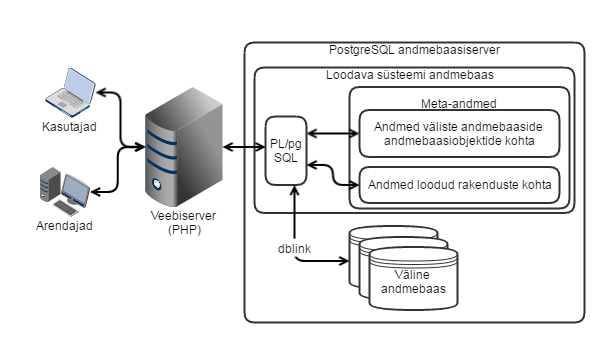
\includegraphics[bb=0 0 604 342,scale=0.75]{./diagrams/how-should-pgapex-work.png}
\caption{Süsteemi tööpõhimõte}
\label{fig_süsteemi_tööpõhimõte}
\end{center}
\end{figure}

\subsection{Litsents}
Üheks töö eesmärgiks oli avaldada loodava prototüübi lähtekood avatud tarkvarana. Olemasolevaid litsentse on väga palju. Selleks, et valida välja litsents, mille all avaldada loodav tarkvara, leian esiteks populaarseimad litsentsid ning võdlen neid omavahel.
GitHub-i poolt avaldatud statistika kohaselt on 2016 aasta märtsi seisuga populaarseimad litsentsid: MIT (44,69\%), GPLv2 (12,96\%), Apache (11,19\%) ja GPLv3 (8,88\%). \cite{GitHub_Opensource_Licence_Usage}\par
Kõik eelpool nimetatud litsentsid täidavad nii \textit{Free Software} (vt Lisa 2) kui ka \textit{Open Source} (vt Lisa 3) tingimusi. Tabelis \ref{table_litsentside_vordlus} on välja toodud litsentside võrdlus.

\begin{table}[H]%[!htb]
\begin{center}
\caption{Litsentside võrdlus}
\label{table_litsentside_vordlus}
\begin{tabular}{|p{3cm}|p{4cm}|p{4cm}|p{4cm}|}
\hline
\rowcolor{rowgray}
 & Nõutud & Lubatud & Keelatud \\ \hline
MIT & Litsents ja copyright märge & Kaubanduslik kasutamine & Võtta vastutusele \\
 &  & Jagamine &  \\
 &  & Muutmine &  \\
 &  & Privaatne kasutamine &  \\ \hline
Apache \newline License 2.0 & Litsents ja copyright märge & Kaubanduslik kasutamine & Võtta vastutusele \\
 & Teavitus muudatustest & Jagamine & Kasutada kaubamärki \\
 &  & Muutmine &  \\
 &  & Patendi kasutamine &  \\
 &  & Privaatne kasutamine &  \\ \hline
GNU GPLv3 & Lähtekoodi avaldamine & Kaubanduslik kasutamine & Võtta vastutusele \\
GNU GPLv2 & Litsents ja copyright märge & Jagamine &  \\
 & Sama litsents & Muutmine &  \\
 & Teavitus muudatustest & Patendi kasutamine &  \\
 &  & Privaatne kasutamine & \\ \hline
\end{tabular}
\cite{Licences}
\end{center}
\end{table}
Valitud sai MIT litsents, kuna see seab kasutajatele kõige vähem piiranguid ning arendajale kõige vähem kohustusi.
\section{Süsteemi analüüs}
\subsection{Tegutsejad}
\begin{itemize}
\item Arendaja.
\item Kasutaja.
\end{itemize}
Arendaja on laiendatud õigustega kasutaja, kellele on lubatud hallata süsteemis loodud rakendusi.
\subsection{Terviksüsteemi tükeldus allsüsteemideks}
Loodav süsteem jagatakse allsüsteemideks, et oleks lihtsam modulaarselt arendada ning struktureeritult kirjeldada loodavat funktsionaalsust.
\subsubsection{Pädevusalad}
\begin{itemize}
\item Arendaja pädevusala.
\item Kasutaja pädevusala.
\end{itemize}
Arendaja pädevusala kasutab kõiki allsüsteeme.\par
Kasutaja pädevusala kasutab ainult rakenduse allsüsteemi.
\subsubsection{Funktsionaalsed allsüsteemid}
\begin{itemize}
\item Rakenduse funktsionaalne allsüsteem.
\item Rakenduste funktsionaalne allsüsteem.
\item Lehtede funktsionaalne allsüsteem.
\item Regioonide funktsionaalne allsüsteem.
\item Navigatsioonide funktsionaalne allsüsteem.
\item Mallide funktsionaalne allsüsteem.
\end{itemize}
Antud töös ei realiseerita mallide funktsionaalset allsüsteemi, kuna töö maht läheks liiga suureks ning loodav süsteem on kasutatav ka ilma selleta.
\subsubsection{Registrid}
\begin{itemize}
\item Andmebaasiobjektide register.
\item Rakenduste register.
\item Lehtede register.
\item Regioonide register.
\item Navigatsioonide register.
\item Mallide register.
\end{itemize}

\subsection{Rakenduse funktsionaalne allsüsteem}
\subsubsection{Eesmärgid}
\begin{itemize}
\item Võimaldada arendajal ja kasutajal kasutada loodud rakendust.
\end{itemize}
\subsubsection{Allsüsteemi poolt kasutatavad registrid}
Allsüsteem ei teeninda ühtegi registrit.\par
Allsüsteem kasutab andmebaasiobjektide registrit, rakenduste registrit, lehtede registrit, regioonide registrit, navigatsioonide registrit ja mallide registrit.
\subsubsection{Allsüsteemi kasutusjuhtude eskiismudel}
Järgnevalt on esitatud rakenduse funktsionaalse allsüsteemi kasutusjuhtude eskiismudel (vt Joonis \ref{fig_rakenduse_funktsionaalse_allsüsteemi_kasutusjuhtude_eskiismudel}) ja seal esitatud kasutusjuhtude tekstikirjeldused kõrgtaseme formaadis.
\begin{figure}[H]
\begin{center}
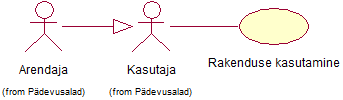
\includegraphics[bb=0 0 346 101,scale=1]{./diagrams/application-subsystem-use-case-digram.png}
\caption{Rakenduse funktsionaalse allsüsteemi kasutusjuhtude eskiismudel}
\label{fig_rakenduse_funktsionaalse_allsüsteemi_kasutusjuhtude_eskiismudel}
\end{center}
\end{figure}

\underline{\textbf{Kasutusjuht:} Rakenduse kasutamine}
\par
\textbf{Tegutsejad:} Arendaja, Kasutaja
\par
\textbf{Kirjeldus:} Kasutaja saab kasutada loodud rakendust. Kasutajale kuvatakse aktiivse lehekülje nähtavate regioonide sisu. Lehel võidakse kuvada navigatsioone, raporteid, vorme ja HTML teksti. Lehtede vahel saab liikuda klikates navigatsiooniregiooni poolt kuvatavatele linkidele. Kui lehekülg pole valitud, siis suutatakse kasutaja avalehele. Kui rakenduses kuvatav lehekülg nõuab, et kasutaja oleks autenditud, siis kuvatakse kasutajale autentimisvorm, kus küsitakse kasutajanime ja parooli. Kui kasutaja poolt sisestatud kasutajanimi ja parool on korrektsed, siis lubatakse kasutajal näha kaitstud lehekülgi. Sessiooni jooksul peab autentima ainult ühe korra.
\par

\subsection{Rakenduste funktsionaalne allsüsteem}
\subsubsection{Eesmärgid}
\begin{itemize}
\item Võimaldada arendajal saada ülevaade loodud rakendustest.
\item Võimaldada arendajal luua uus rakendus.
\item Võimaldada arendajal muuta olemasolevate rakenduste seadeid.
\item Võimaldada arendajal kustutada olemasolevaid rakendusi.
\item Võimaldada arendajal muuta rakenduse autentimismeetodit.
\end{itemize}
\subsubsection{Allsüsteemi poolt kasutatavad registrid}
Allsüsteem teenindab rakenduste registrit.\par
Allsüsteem kasutab andmebaasiobjektide registrit.\par
Allsüsteem kasutab mallide registrit.
\subsubsection{Allsüsteemi kasutusjuhtude eskiismudel}
Järgnevalt on esitatud rakenduste funktsionaalse allsüsteemi kasutusjuhtude eskiismudel (vt Joonis \ref{fig_rakenduste_funktsionaalse_allsüsteemi_kasutusjuhtude_eskiismudel}) ja seal esitatud kasutusjuhtude tekstikirjeldused kõrgtaseme formaadis.
\begin{figure}[H]
\begin{center}
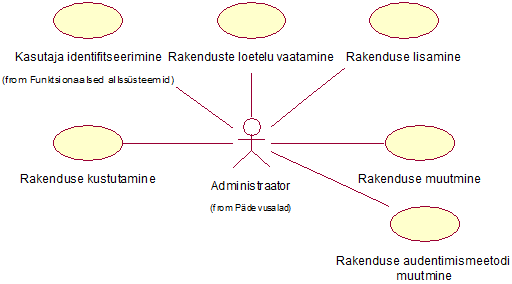
\includegraphics[bb=0 0 512 284,scale=1]{./diagrams/applications-subsystem-use-case-digram.png}
\caption{Rakenduste funktsionaalse allsüsteemi kasutusjuhtude eskiismudel}
\label{fig_rakenduste_funktsionaalse_allsüsteemi_kasutusjuhtude_eskiismudel}
\end{center}
\end{figure}
\underline{\textbf{Kasutusjuht:} Kasutaja identifitseerimine}
\par
\textbf{Tegutsejad:} Arendaja
\par
\textbf{Kirjeldus:} Arendaja identifitseerib ennast sisestades kasutajanime ja parooli. Kui sellise kasutajanime ja parooliga kasutaja on andmebaasis olemas ning kasutajal on SUPERUSER õigused, siis lubatakse arendajal süsteemi siseneda, vastasel juhul mitte.
\par
\textit{Märkus:} Kasutusjuht  ``Kasutaja identifitseerimine'' on kasutusel ka järgnevates allsüsteemides: lehtede funktsionaalne allsüsteem, regioonide funktsionaalne allsüsteem, navigatsioonide funktsionaalne allsüsteem.\par

\underline{\textbf{Kasutusjuht:} Rakenduste loetelu vaatamine}
\par
\textbf{Tegutsejad:} Arendaja
\par
\textbf{Kirjeldus:} Arendaja tahab saada ülevaadet, mis rakendused on loodud. Süsteem kuvab arendajale loetelu rakendustest, kus on esitatud rakenduse nimi.
\par

\underline{\textbf{Kasutusjuht:} Rakenduse lisamine}
\par
\textbf{Tegutsejad:} Arendaja
\par
\textbf{Kirjeldus:} Arendaja tahab luua uue rakenduse. Arendaja valib rakendusele nime, aliase, andmebaasi, mille põhjal rakendus luuakse ning sisestab andmebaasi kasutajanime ja parooli, kellena süsteem andmebaasiga suhtleb. Kui sisestatud andmed on korrektsed ning sellise kasutajanime ja parooliga kasutaja eksisteerib, siis luuakse uus rakendus. Vigade korral kuvatakse vastavad veateated.
\par

\underline{\textbf{Kasutusjuht:} Rakenduse muutmine}
\par
\textbf{Tegutsejad:} Arendaja
\par
\textbf{Kirjeldus:} Arendaja valib rakenduse, mida ta soovib muuta. Arendajale kuvatakse rakenduse nimi, alias, andmebaas, mille põhjal rakendus on loodud ning andmebaasi kasutajanimi. Arendaja saab kuvatud andmeid muuta. Salvestamiseks peab ta sisestama ka andmebaasi kasutajale vastava parooli. Kui sisestatud andmed on korrektsed, siis muudatused salvestatakse. Vigade korral kuvatakse vastavad veateated.
\par

\underline{\textbf{Kasutusjuht:} Rakenduse kustutamine}
\par
\textbf{Tegutsejad:} Arendaja
\par
\textbf{Kirjeldus:} Arendaja valib rakenduse, mida ta soovib kustutada. Enne kustutamist küsitakse arendajalt kinnitust. Kui arendaja kinnitab kustutamise, siis rakendus ning sellega seotud info kustutatakse.
\par

\underline{\textbf{Kasutusjuht:} Rakenduse autentimismeetodi muutmine}
\par
\textbf{Tegutsejad:} Arendaja
\par
\textbf{Kirjeldus:} Arendaja valib rakenduse, mille autentimismeetodit ta soovib muuta. Arendajale kuvatakse hetkel kasutusel olev autentimismeetod koos autentimisfunktsiooniga ning sisselogmislehe malliga. Arendaja saab eelpool nimetatud andmeid muuta.
\par

\subsection{Lehtede funktsionaalne allsüsteem}
\subsubsection{Eesmärgid}
\begin{itemize}
\item Võimaldada arendajal saada ülevaade rakendusele kuuluvatest lehtekülgedest.
\item Võimaldada arendajal luua uusi lehekülgi.
\item Võimaldada arendajal muuta olemasolevate lehekülgede seadeid.
\item Võimaldada arendajal kustutada olemasolevaid lehekülgi.
\end{itemize}
\subsubsection{Allsüsteemi poolt kasutatavad registrid}
Allsüsteem teenindab lehtede registrit.\par
Allsüsteem kasutab mallide registrit.
\subsubsection{Allsüsteemi kasutusjuhtude eskiismudel}
Järgnevalt on esitatud lehtede funktsionaalse allsüsteemi kasutusjuhtude eskiismudel (vt Joonis \ref{fig_lehtede_funktsionaalse_allsüsteemi_kasutusjuhtude_eskiismudel}) ja seal esitatud kasutusjuhtude tekstikirjeldused kõrgtaseme formaadis.
\begin{figure}[H]
\begin{center}
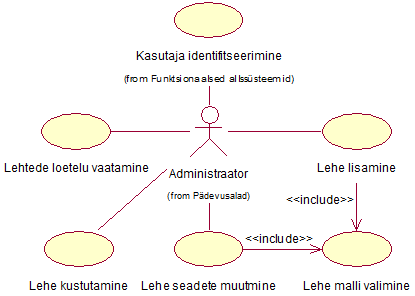
\includegraphics[bb=0 0 395 203,scale=1]{./diagrams/pages-subsystem-use-case-digram.png}
\caption{Lehtede funktsionaalse allsüsteemi kasutusjuhtude eskiismudel}
\label{fig_lehtede_funktsionaalse_allsüsteemi_kasutusjuhtude_eskiismudel}
\end{center}
\end{figure}

\underline{\textbf{Kasutusjuht:} Lehtede loetelu vaatamine}
\par
\textbf{Tegutsejad:} Arendaja
\par
\textbf{Kirjeldus:} Arendaja tahab saada ülevaadet, mis leheküljed on rakenduse alla loodud. Süsteem kuvab arendajale loetelu lehtedest, kus tuuakse välja lehe id, alias, pealkiri ja info selle kohta, kas leht on avaleht ning kas leht nõuab kasutaja autentimist.
\par

\underline{\textbf{Kasutusjuht:} Lehe lisamine}
\par
\textbf{Tegutsejad:} Arendaja
\par
\textbf{Kirjeldus:} Arendaja tahab luua rakenduse alla uue lehe. Arendaja sisestab lehe pealkirja, aliase, valib lehe malli, mida kasutatakse lehe kuvamisel ja valib kas leht on avaleht ning kas leht nõuab autentimist. Kui andmed on korrektsed, siis luuakse uus leht. Vastasel korral kuvatakse vastavad veateated.
\par

\underline{\textbf{Kasutusjuht:} Lehe seadete muutmine}
\par
\textbf{Tegutsejad:} Arendaja
\par
\textbf{Kirjeldus:} Arendaja valib lehtede loetelust lehe, mida ta soovib muuta. Arendajale kuvatakse lehe pealkiri, alias, mall ja info selle kohta kas tegu on avalehega ning kas leht nõuab kasutaja autentimist. Kuvatavaid andmeid saab muuta. Kui andmed on korraktsed, siis need salvestatakse. Vastasel korral kuvatakse vastavad veateated.
\par

\underline{\textbf{Kasutusjuht:} Lehe kustutamine}
\par
\textbf{Tegutsejad:} Arendaja
\par
\textbf{Kirjeldus:} Arendaja valib lehtede loetelust lehe, mida ta soovib kustutada. Enne kustutamist küsitakse arendajalt kinnitust. Kui arendaja kinnitab kustutamise, siis leht ning sellega seotud info kustutatakse.
\par

\subsection{Regioonide funktsionaalne allsüsteem}
\subsubsection{Eesmärgid}
\begin{itemize}
\item Võimaldada arendajal saada ülevaade lehel olevatest regioonidest.
\item Võimaldada arendajal luua navigatsiooni tüüpi regioone.
\item Võimaldada arendajal luua HTML tüüpi regioone.
\item Võimaldada arendajal luua raporti tüüpi regioone.
\item Võimaldada arendajal luua vormi tüüpi regioone.
\item Võimaldada arendajal muuta olemasolevaid regioone.
\item Võimaldada arendajal kustutada olemasolevaid regioone.
\end{itemize}
\subsubsection{Allsüsteemi poolt kasutatavad registrid}
Allsüsteem teenindab regioonide registrit.\par
Allsüsteem kasutab mallide registrit, navigatsioonide registrit, andmebaasiobjektide registrit.
\subsubsection{Allsüsteemi kasutusjuhtude eskiismudel}
Järgnevalt on esitatud regioonide funktsionaalse allsüsteemi kasutusjuhtude eskiismudel (vt Joonis \ref{fig_regioonide_funktsionaalse_allsüsteemi_kasutusjuhtude_eskiismudel}) ja seal esitatud kasutusjuhtude tekstikirjeldused kõrgtaseme formaadis.
\begin{figure}[H]
\begin{center}
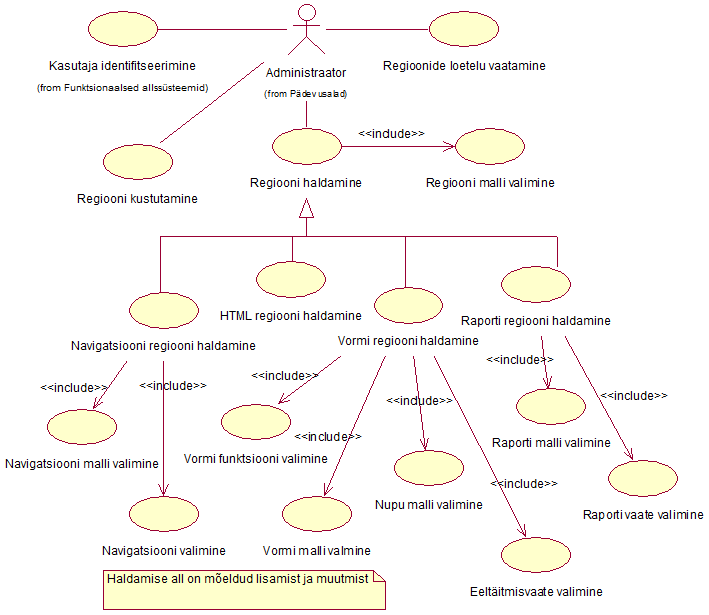
\includegraphics[bb=0 0 531 399,scale=1]{./diagrams/regions-subsystem-use-case-digram.png}
\caption{Regioonide funktsionaalse allsüsteemi kasutusjuhtude eskiismudel}
\label{fig_regioonide_funktsionaalse_allsüsteemi_kasutusjuhtude_eskiismudel}
\end{center}
\end{figure}

\underline{\textbf{Kasutusjuht:} Regioonide loetelu vaatamine}
\par
\textbf{Tegutsejad:} Arendaja
\par
\textbf{Kirjeldus:} Arendaja tahab saada ülevaadet, mis regioonid on valitud lehe alla loodud. Arendajale kuvatakse regioonide loetelu, kus esitatakse regiooni asukoht lehel, regiooni tüüp, järjekorranumber, nimi ning info selle kohta, kas regioon on nähtav või peidetud.
\par

\underline{\textbf{Kasutusjuht:} Regiooni kustutamine}
\par
\textbf{Tegutsejad:} Arendaja
\par
\textbf{Kirjeldus:} Arendaja valib regioonide loetelust regiooni, mida ta soovib kustutada. Enne kustutamist küsitakse arendajalt kinnitust. Kui arendaja kinnitab kustutamise, siis regioon ning sellega seotud info kustutatakse.

\underline{\textbf{Kasutusjuht:} Regiooni haldamine}
\par
\textbf{Tegutsejad:} Arendaja
\par
\textbf{Kirjeldus:} Regiooni lisamisel või muutmisel kuvatakse arendajale vorm, kus küsitakse regiooni nime, järjekorranumbrit, regiooni malli, mida kasutatakse regiooni kuvamisel ning infot selle kohta, kas regioon on nähtav või peidetud. Regiooni muutmise korral on vormi väljad eelnevalt täidetud. Kui esitatud andmed on korrektsed, siis need salvestatakse. Vastasel korral kuvatakse vastavad veateated.

\underline{\textbf{Kasutusjuht:} HTML regiooni haldamine}
\par
\textbf{Tegutsejad:} Arendaja
\par
\textbf{Kirjeldus:} HTML regiooni lisamisel või muutmisel kuvatakse arendajale vorm, kus lisaks kasutusjuhus ``Regiooni haldamine'' esitatud andmetele küsitakse arendajalt ka teksti, mida regioonis kuvada.

\underline{\textbf{Kasutusjuht:} Navigatsiooni regiooni haldamine}
\par
\textbf{Tegutsejad:} Arendaja
\par
\textbf{Kirjeldus:} Navigatsiooni regiooni lisamisel või muutmisel kuvatakse arendajale vorm, kus lisaks kasutusjuhus ``Regiooni haldamine'' esitatud andmetele küsitakse arendajalt ka navigatsiooni malli, kuvamise tüüpi ja navigatsiooni, mille alusel regioon luuakse ning infot selle kohta, kas regiooni kuvamisel tuleb korrata navigatsioonipunkti malli viimast taset, juhul kui navigatsioonipunkti sügavuse jaoks pole eraldi malli defineeritud.

\underline{\textbf{Kasutusjuht:} Raporti regiooni haldamine}
\par
\textbf{Tegutsejad:} Arendaja
\par
\textbf{Kirjeldus:} Raporti regiooni lisamisel või muutmisel kuvatakse arendajale vorm, kus lisaks kasutusjuhus ``Regiooni haldamine'' esitatud andmetele küsitakse arendajalt ka raporti kuvamisel kasutatavat malli, raporti aluseks olevat vaadet, infot selle kohta, kas raporti päist tuleb kuvada või mitte, mitu rida kuvatakse ühel leheküljel, mis URL-parameetriga antakse edasi hetkel aktiivset lehekülge ning mis veergudest raport koosneb. Pärast vaate valimist saab luua raportile veerge. Raporti veerg võib olla kas valitud vaate veerg või link. Raporti veeru loomisel tuleb sisestada veeru pealkiri, järjekorranumber ning info selle kohta, kas kuvatavas tekstis muudetakse HTML-erimärgid (\&, <, >, ", ') ohutuks või mitte. Lingi korral tuleb lisaks sisestada ka URL ja ning lingi tekst ning võib lisada lisaatribuudid lingi vormindamiseks. Raport peab sisaldama vähemalt ühte veergu.

\underline{\textbf{Kasutusjuht:} Vormi regiooni haldamine}
\par
\textbf{Tegutsejad:} Arendaja
\par
\textbf{Kirjeldus:} Vormi regiooni lisamisel või muutmisel kuvatakse arendajale vorm, kus lisaks kasutusjuhus ``Regiooni haldamine'' esitatud andmetele küsitakse arendajalt ka vormi kuvamisel kasutatavat malli, vormi saatmisnupu malli, saatmisnupul kuvatavat teksti, teadet, mida kuvatakse vormi eduka töötlemise korral, teadet, mida kuvatakse, kui vormi töötlemisel tekib viga, URL, kuhu pärast vormi edukat töötlemist edasi suunatakse, funktsiooni, mille alusel vorm luuakse ning info selle kohta, kas vorm tuleb eelnevalt andmetega täita. Pärast funktsiooni valimist kuvatakse funktsiooni parameetrid ning arendaja peab valima, kuidas neid vormis kuvatakse. Arendaja peab sisestama vormi välja nime, kirjelduse, järjekorranumbri, valima välja tüübi ja malli. Lisaks saab ta valida, kas väli on kogustuslik või mitte, nähtav või peidetud, sisestada välja vaikimisi väärtuse ja kasutajat abistava teksti. Juhul kui välja tüübiks on mitme valikuvõimalusega element, siis peab kasutaja valima vaate ja veerud, mille põhjal valikud luuakse. Juhuk kui on valitud vaade, mille põhjal vorm eeltäidetakse, siis peab arendaja ära kirjeldama päringu tingimused, mille alusel leitakse vaatest õige rida ning määrama, millised vormi väljad infoga täidetakse.

\subsection{Navigatsioonide funktsionaalne allsüsteem}
\subsubsection{Eesmärgid}
\begin{itemize}
\item Võimaldada arendajal saada ülevaade rakendusele kuuluvatest navigatsioonidest.
\item Võimaldada arendajal luua uusi navigatsioone.
\item Võimaldada arendajal muuta olemasolevate navigatsioone.
\item Võimaldada arendajal kustutada olemasolevaid navigatsioone.
\item Võimaldada arendajal lisada olemasoleva navigatsiooni alla navigatsioonipunkte.
\item Võimaldada arendajal muuta olemasolevaid navigatsioonipunkte.
\item Võimaldada arendajal kustutada olemasolevaid navigatsioonipunkte.
\end{itemize}
\subsubsection{Allsüsteemi poolt kasutatavad registrid}
Allsüsteem teenindab navigatsioonide registrit.\par
Allsüsteem kasutab lehtede registrit.
\subsubsection{Allsüsteemi kasutusjuhtude eskiismudel}
Järgnevalt on esitatud navigatsioonide funktsionaalse allsüsteemi kasutusjuhtude eskiismudel (vt Joonis \ref{fig_navigatsioonide_funktsionaalse_allsüsteemi_kasutusjuhtude_eskiismudel}) ja seal esitatud kasutusjuhtude tekstikirjeldused kõrgtaseme formaadis.
\begin{figure}[H]
\begin{center}
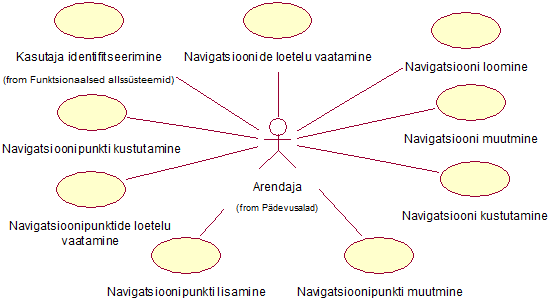
\includegraphics[bb=0 0 553 306,scale=1]{./diagrams/navigations-subsystem-use-case-digram.png}
\caption{Navigatsioonide funktsionaalse allsüsteemi kasutusjuhtude eskiismudel}
\label{fig_navigatsioonide_funktsionaalse_allsüsteemi_kasutusjuhtude_eskiismudel}
\end{center}
\end{figure}

\underline{\textbf{Kasutusjuht:} Navigatsioonide loetelu vaatamine}
\par
\textbf{Tegutsejad:} Arendaja
\par
\textbf{Kirjeldus:} Arendaja tahab saada ülevaadet, mis navigatsioonid on valitud rakenduse alla loodud. Arendajale kuvatakse navigatsioonide nimede loetelu.
\par

\underline{\textbf{Kasutusjuht:} Navigatsiooni loomine}
\par
\textbf{Tegutsejad:} Arendaja
\par
\textbf{Kirjeldus:} Arendaja tahab luua uut navigatsiooni. Arendajale kuvatakse vorm, kus küsitakse uue navigatsiooni nime. Kui sisestatud andmed on korrektsed, siis luuakse navigatsioon. Vastasel korral kuvatakse vastvad veateated.
\par

\underline{\textbf{Kasutusjuht:} Navigatsiooni muutmine}
\par
\textbf{Tegutsejad:} Arendaja
\par
\textbf{Kirjeldus:} Arendaja valib navigatsiooni, mida ta soovib muuta. Arendajale kuvatakse navigatsiooni nimi. Kuvatavaid andmeid saab muuta. Kui andmed on korraktsed, siis need salvestatakse. Vastasel korral kuvatakse vastavad veateated.
\par

\underline{\textbf{Kasutusjuht:} Navigatsiooni kustutamine}
\par
\textbf{Tegutsejad:} Arendaja
\par
\textbf{Kirjeldus:} Arendaja valib navigatsioonide loetelust navigatsiooni, mida ta soovib kustutada. Enne kustutamist küsitakse arendajalt kinnitust. Kui arendaja kinnitab kustutamise, siis navigatsioon ning sellega seotud info kustutatakse.
\par

\underline{\textbf{Kasutusjuht:} Navigatsioonipunktide loetelu vaatamine}
\par
\textbf{Tegutsejad:} Arendaja
\par
\textbf{Kirjeldus:} Arendaja tahab saada ülevaadet, millised navigatsioonipunktid on navigatsiooni alla loodud. Arendajale kuvatakse loetelu navigatsioonipunktidest, kus on esitatud navigatsioonipunkti järjekorranumber, nimi ja URL või leht, millele ta viitab. Lisaks on välja toodud, millise navigatsioonipunkti alla ta kuulub.
\par

\underline{\textbf{Kasutusjuht:} Navigatsioonipunkti lisamine}
\par
\textbf{Tegutsejad:} Arendaja
\par
\textbf{Kirjeldus:} Arendaja tahab navigatsiooni alla lisada navigatsioonipunkti. Arendajale kuvatakse vorm, kus küsitakse navigatsioonipunkti nime, järjekorranumbrit, ülem-navigatsioonipunkti ning URL-i või lehte, millele viidatakse. Kui sisestatud andmed on korrektsed, siis luuakse uus navigatsioonipunkt. Vastasel korral kuvatakse vastavad veateated.
\par

\underline{\textbf{Kasutusjuht:} Navigatsioonipunkti muutmine}
\par
\textbf{Tegutsejad:} Arendaja
\par
\textbf{Kirjeldus:} Arendaja tahab muuta olemasolevat navigatsioonipunkti. Arendajale kuvtakse vorm, kus esitatakse olemasoleva navigatsioonipunkti nimi, järjekorranumber, ülem-navigatsioonipunkt ning URL või leht, millele viidatakse. Arendaja saab muuta eelpool nimetatud andmeid. Kui andmed on korrektsed, siis andmed salvestatakse. Vastasel korral kuvatakse vastavad veateated.
\par

\underline{\textbf{Kasutusjuht:} Navigatsioonipunkti kustutamine}
\par
\textbf{Tegutsejad:} Arendaja
\par
\textbf{Kirjeldus:} Arendaja valib navigatsioonipunktide loetelust navigatsioonipunkti, mida ta soovib kustutada. Enne kustutamist küsitakse arendajalt kinnitust. Kui arendaja kinnitab kustutamise, siis navigatsioonipunkt ning sellega seotud info kustutatakse.
\par

\subsection{Mittefunktsionaalsed nõuded}
Tabelis \ref{mittefunktsionaalsed_nõuded} on välja toodud süsteemile esitatud mittefunktsionaalsed nõuded, mida loodav süsteem peab täitma.
\begin{table}[H]%[!htb]
\begin{center}
\caption{Mittefunktsionaalsed nõuded}
\label{mittefunktsionaalsed_nõuded}
\begin{tabular}{|p{5cm}|p{10cm}|}
\hline
\rowcolor{rowgray}
Tüüp & Nõude kirjeldus \\ \hline
Serveri tarkvara & Andmete hoidmiseks peab kasutama andmebaasisüsteemi PostgreSQL 9.4 või uuemat. Rakendus tuleb luua kasutades PHP 5.5.0 või uuemat. \\ \hline
Keel & Süsteemi kasutajaliides peab olema ingliskeelne. \\ \hline
Kasutajaliides & Kasutajaliides peab olema veebipõhine ning arvestama erinevate resolutsioonidega. \\ \hline
Toetatud veebibrauserid & 
\begin{itemize}
\item Microsoft Internet Explorer 11 või uuem.
\item Mozilla Firefox 43 või uuem.
\item Google Chrome 49 või uuem.
\end{itemize}
 \\ \hline
Andmebaasioperatsioonide töökiirus & Andmebaasioperatsioonid peavad süsteemil aega võtma alla 5 sekundi. \\ \hline
\end{tabular}
\end{center}
\end{table}

\section{Andmebaas}
Järgnevalt esitatakse loodava süsteemi andmemudeli olemi-suhte diagrammid registrite kaupa ning kirjeldatakse, mille jaoks vastavaid olemitüüpe ning atribuute vaja läheb. Punasega on tähistatud registri põhiobjekt, kollasega registrisse kuuluvad mitte-põhiobjektid ning rohelisega teistesse registritesse kuuluvad objektid, mida vaadeldav register vajab. Diagrammidel on objektid kirjeldatud inglise keeles, kuna nende põhjal genereeriti tabelid ning lootes, et loodav süsteem leiab laiemat kasutust, siis oleks kasulik, kui süsteemi poolt kasutatavad osad oleks kirjutatud inglise keeles. Olemi-suhte diagrammide põhjal genereeritud tabelid on Lisas X.

\subsection{Andmebaasiobjektide register}
\begin{figure}[H]
\begin{center}
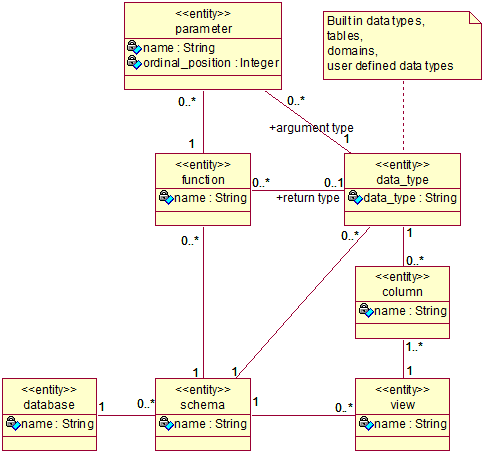
\includegraphics[bb=0 0 485 456,scale=1]{./diagrams/database-object-er-diagram.png}
\caption{Andmebaasiobjektide registri olemi-suhte diagramm}
\label{fig_andmebaasiobjektide_registri_olemi_suhte_diagramm}
\end{center}
\end{figure}

\subsection{Rakenduste register}
\begin{figure}[H]
\begin{center}
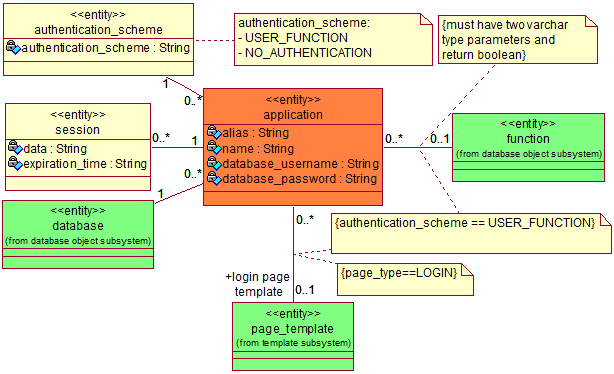
\includegraphics[bb=0 0 614 374,scale=1]{./diagrams/applications-er-diagram.png}
\caption{Rakenduste registri olemi-suhte diagramm}
\label{fig_rakenduste_registri_olemi_suhte_diagramm}
\end{center}
\end{figure}

\subsection{Lehtede register}
\begin{figure}[H]
\begin{center}
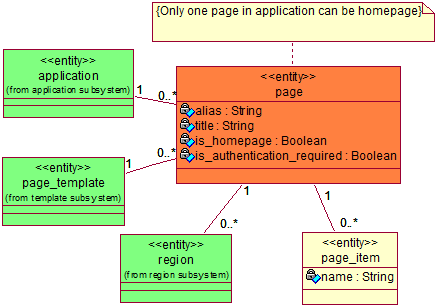
\includegraphics[bb=0 0 438 307,scale=1]{./diagrams/page-er-diagram.png}
\caption{Lehtede registri olemi-suhte diagramm}
\label{fig_lehtede_registri_olemi_suhte_diagramm}
\end{center}
\end{figure}


\subsection{Regioonide register}
\begin{figure}[H]
\begin{center}
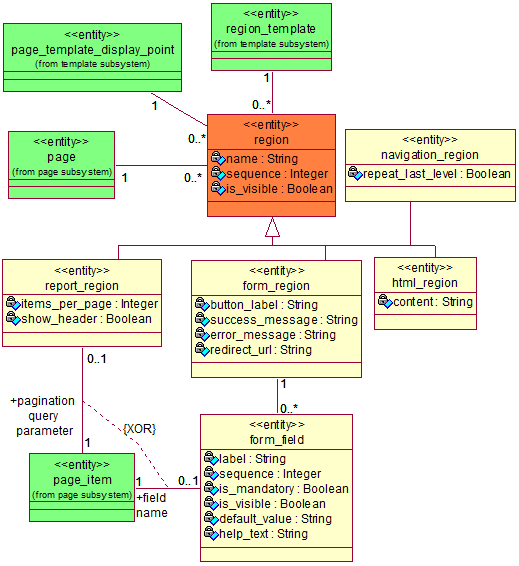
\includegraphics[bb=0 0 519 566,scale=1]{./diagrams/region-er-diagram.png}
\caption{Regioonide registri olemi-suhte diagramm osa 1}
\label{fig_regioonide_registri_olemi_suhte_diagramm}
\end{center}
\end{figure}

\begin{figure}[H]
\begin{center}
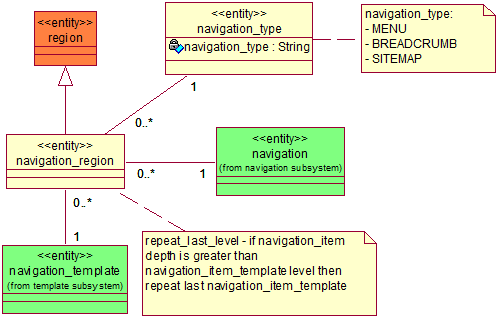
\includegraphics[bb=0 0 360 235,scale=1]{./diagrams/navigation-region-er-diagram.png}
\caption{Regioonide registri olemi-suhte diagramm osa 2}
\label{fig_navigatsiooni_regioonide_registri_olemi_suhte_diagramm}
\end{center}
\end{figure}

\begin{figure}[H]
\begin{center}
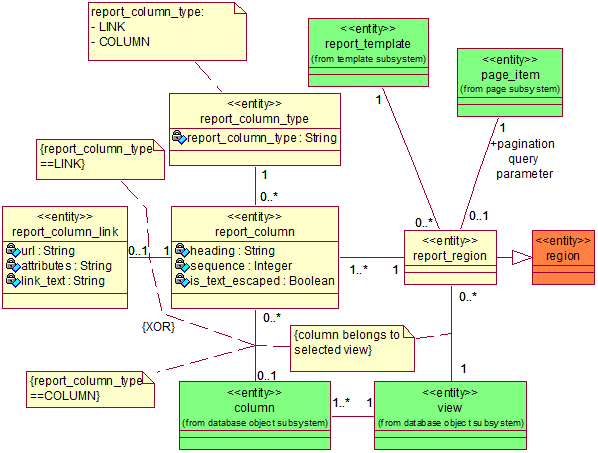
\includegraphics[bb=0 0 575 480,scale=1]{./diagrams/report-region-er-diagram.png}
\caption{Regioonide registri olemi-suhte diagramm osa 3}
\label{fig_raportite_regioonide_registri_olemi_suhte_diagramm}
\end{center}
\end{figure}

\begin{figure}[H]
\begin{center}
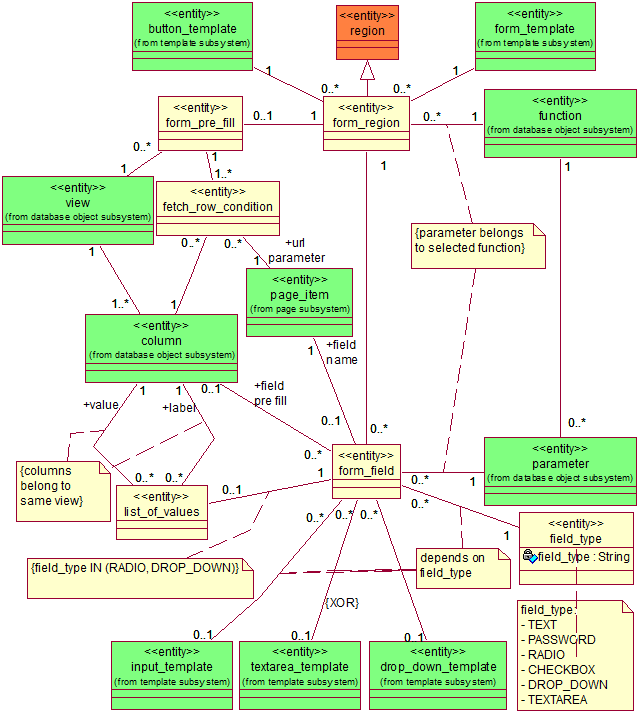
\includegraphics[bb=0 0 640 776,scale=1]{./diagrams/form-region-er-diagram.png}
\caption{Regioonide registri olemi-suhte diagramm osa 4}
\label{fig_vormide_regioonide_registri_olemi_suhte_diagramm}
\end{center}
\end{figure}

\subsection{Navigatsioonide register}
Navigatsioonide register
\begin{figure}[H]
\begin{center}
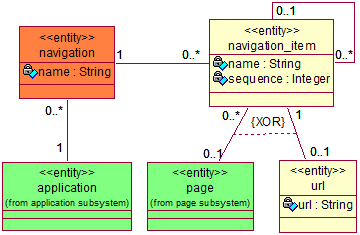
\includegraphics[bb=0 0 360 235,scale=1]{./diagrams/navigation-er-diagram.png}
\caption{Navigatsioonide registri olemi-suhte diagramm}
\label{fig_navigatsioonide_registri_olemi_suhte_diagramm}
\end{center}
\end{figure}

\subsection{Mallide register}
\begin{figure}[H]
\begin{center}
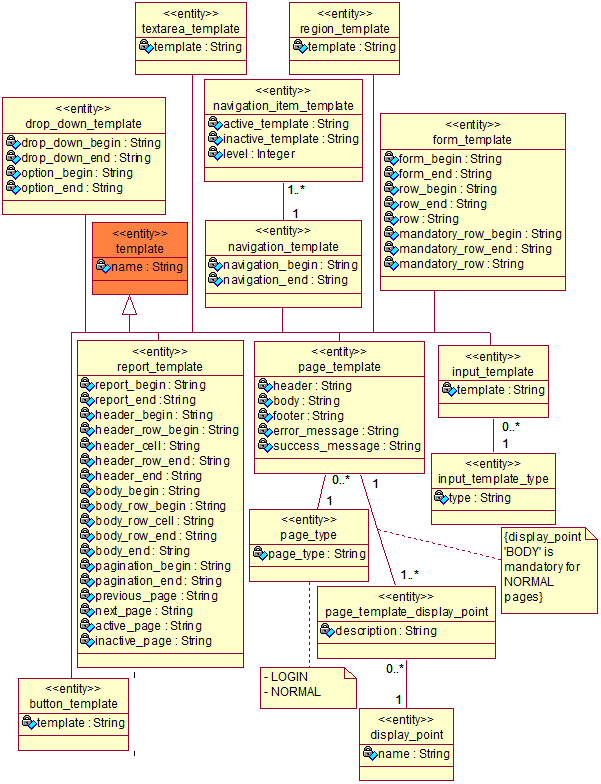
\includegraphics[bb=0 0 601 784,scale=1]{./diagrams/template-er-diagram.png}
\caption{Mallide registri olemi-suhte diagramm}
\label{fig_mallide_registri_olemi_suhte_diagramm}
\end{center}
\end{figure}

\section{Arendusvahendid ja arendusprotsess}
\subsection{Vagrant}
Vagrant on käsureaprogramm, millega saab hallata virtuaalmasina elutsüklit. Vagrant isoleerib programmilised sõltuvused ja nende konfiguratsioonid ühtsesse eraldiseisvasse keskkonda. Keskkonna konfigureerimiseks saab kasutada käsurea käsklusi, \textit{Ansible}-t \cite{Ansible}, \textit{Puppet}-it \cite{Puppet}, \textit{Chef}-i \cite{Chef}, \textit{Docker}-it \cite{Docker} ja \textit{Salt}-i \cite{Salt}. Tänu Vagrantile saavad kõik luua endale täpselt ühesuguse keskkonna, kus programme jooksutada, vähendades võimalust, et ühes arvutis programm jookseb, teises aga mitte. \cite{Why_Vagrant}
\subsection{AngularJS}
Angular on raamistik loomaks dünaamilisi veebirakendusi. See võimaldab laiendada HTML süntaksit, et panna elemendid käituma vastavalt arendaja soovile. Angular kasutab kahe suunalist andmesidumist (\textit{data binding}). See tähendab et muudatused javascripti koodis kajastuvad automaatselt HTML-is ning vastupidi. Tänu sellele peab arendaja vähem tegelema DOM-i manipuleerimisega.  \cite{AngularJS}.
\subsection{Bootstrap}
Bootstrap on mobiilisõbralik kasutajaliidese raamistik, mille abil saab luua dünaamilist veebidisaini (\textit{responsive web design}), mis arvestab kasutaja ekraani suurusega ning kohandab end jooksvalt vastavalt sellele. Bootstrap-is on realiseeritud mitmed komponendid, mis kiirendavad kasutajaliidese loomist. Bootstrap kasutab HTML-i, javascripti js CSS-i. \cite{Bootstrap}
\subsection{Bower}
Bower on paketihaldussüsteem (\textit{package manager}), mis on mõeldud veebis kasutatavate failide, nagu näiteks HTML, CSS, javascript, fondid ja pildid, haldamiseks. Bower-i kasutamiseks peab masinasse olema installitud node, npm ja git. Paketide haldus toimub bower.json failis, kus kirjeldatakse ära soovitud paketid ning nende versioonid. \cite{Bower}
\subsection{TravisCI}
TravisCI on pideva integratsiooni (\textit{continuous integration}) keskkond, mille abil saab luua virtuaalse keskkonna koodi kompilleerimiseks, testimiseks ja juurutamiseks. Keskkonna seadistamine toimub faili .travis.yml abil, kus määratakse ära virtuaalkeskkonna operatsioonisüsteem, teegid, mis tuleb installida ning käivitatavad käsud.
\subsection{Arendusprotsess}
Esimese asjana sai paika pandud esmased nõuded, mida süsteem peaks võimaldama teha. Kuna süsteemi esimene potentsiaalne kasutuskoht oleks TTÜ-s õpetatavas aines ``Andmebaasid II'', siis konsulteeriti antud õppeaine õppejõuga ning kaardistati enim levinud kasutusjuhud, mida antud aine raames tuleb üliõpilastel realiseerida. Kui nõuded olid paigas, siis loodi nende põhjal andmemudel ning kasutajaliidese prototüüp, mis võeti hiljem loodavas süsteemis kasutusele. Prototüüp kasutas andmete kuvamiseks võltsandmeid (\textit{mock data}). See andis hea ettekujutuse loodava süsteemi võimekusest ning aitas juhtida tähelepanu aspektidele, millele ilma prototüübi abita ei oleks kohe tuldud.\par

Selleks et loodavat süsteemi oleks ka teistel arendajatel lihtsam kasutusele võtta ning täiustada sai arenduskeskkonna loomiseks kasutusele võetud Vagrant \cite{Vagrant}, mille abil loodi virtuaalmasin koos kõigi arenduseks vajalike teekidega. Virtuaalmasina konfigureerimiseks kasutati bash-i skripti.\par

Selleks et süsteemi kasutamine oleks sujuv võeti kasutajaliidese loomiseks kasutusele AngularJS 1.4 \cite{AngularJS}. Lihtsustamaks kasutajaliidese ühtset väljanägemist erinevates brauserites ning eri suurustes ekraanidega, kasutati Bootstrap 3 \cite{Bootstrap}. Kasutajaliidese poolt kasutatavaid sõltuvusi hallati \cite{Bower}-i abil. Koodi kvaliteedi kontrollimiseks ja säilitamiseks kirjutati testid, mida jooksutati Karma \cite{Karma} abil.\par

Andmebaasi loomisel lähtuti ideest, et kogu suhtlus andmebaasiga peab käima läbi andmebaasiliidese \ref{andmebaasi_avalik_liides}. Andmete salvestamiseks ning küsimiseks tuleb kasutajal välja kutsuda vastav andmebaasifunktsioon. Kasutamaks ära PostgreSQL-i võimalust väljastada JSON tüüpi andmeid luuakse kasutajaliidese jaoks vajalik vastus juba andmebaasis. Tänu sellele pole andmetega manipuleerimine süsteemis laiali jaotatud vaid toimub üksnes andmebaasi poolel.\par

Andmebaasi ja kasutajaliidese vaheline suhtlus toimub läbi PHP-s \cite{PHP} kirjutatud rakenduse. Kuna antud rakenduse kiht on üpriski õhuke, siis sai selle loomiseks valitud ka lihtsakoeline raamistik Slim Framework 3 \cite{SlimFW}. PHP-s kirjutatud koodi testimiseks kasutati PHPUnit-it \cite{PHPUnit} ning Mockery-t \cite{Mockery}. Koodi sõltuvusi hallati Composer-i abil \cite{Composer}. \par

Koodi hoidmiseks kasutatakse GitHub-i \cite{GitHub}. Iga kord, kui koodihoidlasse midagi üles laetakse luuakse TravisCI-s \cite{TravisCI} virtuaalkeskkond, kuhu tõmmatakse GitHub-st loodava süsteemi kood ning testide eduka jooksutamise korral juurutatakse serverisse. Tänu sellele on serveris alati näha süsteemi viimane töötav version.

\section{Kasutajaliidese disain}
Kasutajaliidese loomiseks kasutas autor 
\section{Rakenduse disain}
\section{Näidisrakendus}
Valideerimaks, kas loodud süsteem vastab nõuetele, loon näiterakenduse ja realiseerin neli kasutusjuhtu (vt Joonis \ref{fig_näidisrakendus_kasutusjuhtude_eskiismudel}), mis sarnanevad üliõpilastöödes esinevatele kasutusjuhtudele. Kasutaja tuvastamine põhineb funktsioonil functions.f\_is\_boss, mille esimese parameetri oodatav väärtus on kasutajanimi ja teise parameetri oodatav väärtus on paool. Kõikide ruumide anmete vaatamine põhineb vaatel public.overview\_of\_rooms. Ruumide koondaruande vaatamine põhineb vaatel public.number\_of\_rooms\_by\_state. Ruumi mitteaktiivseks muutmine põhineb funktsioonil functions.f\_permanently\_inactivate\_a\_room, mille oodatavaks argumendiks on ruumi kood, mis tuleb valida vaatest public.active\_temporariliy\_inactive\_rooms.
\begin{figure}[H]
\begin{center}
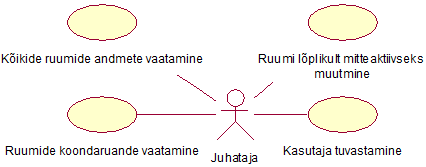
\includegraphics[bb=0 0 430 164,scale=1]{./diagrams/sample-application-use-case-diagram.png}
\caption{Näidisrakenduse kasutusjuhtude eskiismudel}
\label{fig_näidisrakendus_kasutusjuhtude_eskiismudel}
\end{center}
\end{figure}
\subsection{Kasutaja tuvastamine}
Kui kasutaja läheb lehele, mille nägemiseks peab ta olema autenditud, siis kuvatakse talle sisselogimise vorm, kuhu tuleb sisestada kasutajanimi ja parool (vt Joonis \ref{fig_näidisrakendus_kasutaja_tuvastamine}). Kui kasutajanimi ja parool on õiged, siis logitakse kasutaja sisse ning kasutaja näeb edaspidi autentimist nõudvate lehtede sisu.
\begin{figure}[H]
\begin{center}
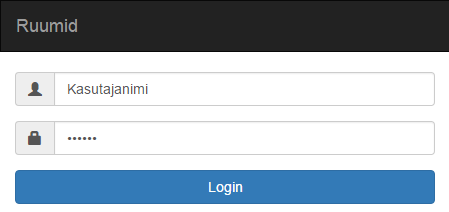
\includegraphics[bb=0 0 449 212,scale=1]{./diagrams/sample-app-user-auth.png}
\caption{Kasutaja tuvastamine}
\label{fig_näidisrakendus_kasutaja_tuvastamine}
\end{center}
\end{figure}
\subsection{Ruumide koondaruande ja kõikide ruumide vaatamine}
Kasutajale kuvatakse ühel lehel nii ruumide koondaruanne kui ka kõikide ruumide info, kusjuures raportite read on võimalik jaotada lehekülgedele (vt Joonis \ref{fig_näidisrakendus_raportid})
\begin{figure}[H]
\begin{center}
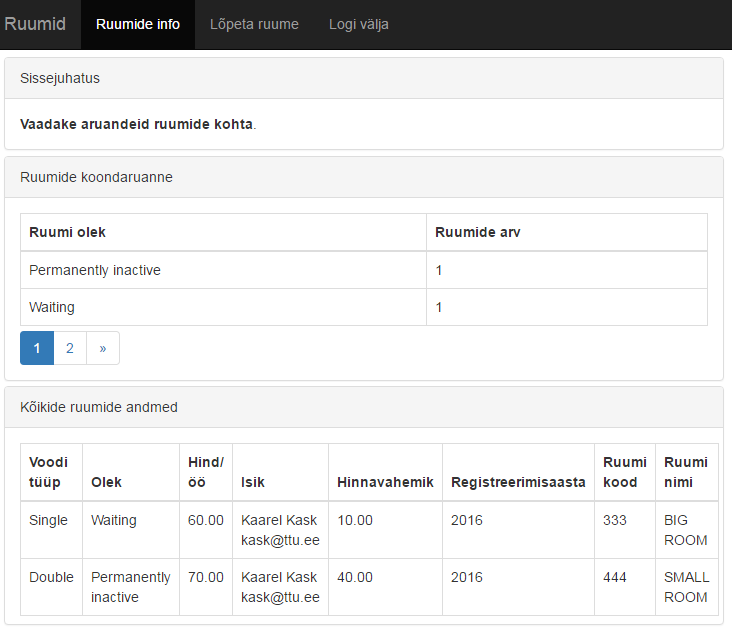
\includegraphics[bb=0 0 732 630,scale=0.8]{./diagrams/sample-app-reports.png}
\caption{Ruumide koondaruande ja kõikide ruumide vaatamine}
\label{fig_näidisrakendus_raportid}
\end{center}
\end{figure}
\subsection{Ruumi lõplikult mitteaktiivseks muutmine}
Kasutajale kuvatakse vorm, kus kust ta saab valida millist ruumi ta muuta soovib (vt Joonis \ref{fig_näidisrakendus_vorm}). Ruumide loetelu saadakse vaate  public.active\_temporariliy\_inactive\_rooms põhjal. Pärast vormi saatmist kutsutakse välja funktsioon functions.f\_permanently\_inactivate\_a\_room. Kui funktsiooni lõpetab oma töö ilma vigadeta, siis tagastatakse kasutajale teade, et vormi saatmine õnnestus.
\begin{figure}[H]
\begin{center}
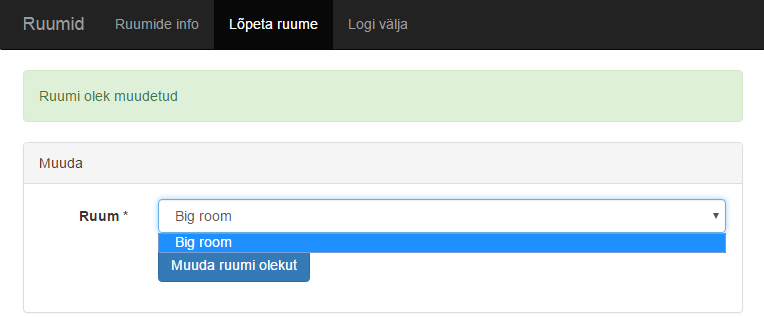
\includegraphics[bb=0 0 764 317,scale=0.8]{./diagrams/sample-app-form.png}
\caption{Ruumi lõplikult mitteaktiivseks muutmine}
\label{fig_näidisrakendus_vorm}
\end{center}
\end{figure}

%-------------------------------KOKKUVÕTE---------------------------
\section{Kokkuvõte}
Kokkuvõte

\pagebreak

\section{Summary}
Kokkuvõte

\pagebreak

%------------------------------KASUTATUD KIRJANDUS-----------------------------------
\addcontentsline{toc}{section}{Kasutatud kirjandus}
\bibliographystyle{plain}
\bibliography{pgapex}

\pagebreak

%-----------------------------LISAD--------------------------------
\section*{Lisa 1 - PostgreSQL andmabaasisüsteemi süsteemikataloogid}
\label{lisa1}
\addcontentsline{toc}{section}{Lisa 1}
\subsection{information\_schema}
\begin{labeling}{element\_types}
\item [schemata] Sisaldab kõiki skeeme, millele kasutajal on ligipääs.
\item [views] Sisaldab kõiki vaateid, mis asuvad antud andmebaasis. Näidatakse ainult selliseid vaateid, millele kasutajal on ligipääs. Paraku ei saa sealt aga infot materialiseeritud vaadete kohta.
\item [columns] Sisaldab infot andmebaasis olevate tabelite ja vaadete veergude kohta. Näidatakse ainult neid veerge, millele kasutajal on ligipääs. Kui tagastatav tüüp on massiiv, siis saab selle kohta infot information\_schema.element\_types vaatest. Kui tagastatav tüüp on USER-DEFINED, siis saab selle kohta infot udt\_name veerust. Kui veerg on loodud domeeni põhjal, siis saab domeeni nime domain\_name veerust
\item [routines] Sisaldab infot andmebaasis olevate funktsioonide kohta, millele kasutajal on ligipääs. data\_type veerg sisaldab infot tagastatava tüübi kohta. Kui tagastatav tüüp on massiiv, siis saab selle kohta infot information\_schema.element\_types vaatest. Kui tagastatav tüüp on USER-DEFINED, siis saab selle kohta infot type\_udt\_name veerust.
\item [parameters] Sisaldab infot andmabaasis olevate funktsioonide parameetrite kohta. Parameetreid näidatakse ainult nende funktsioone kohta, millele kasutajal on ligipääs.
\item [element\_types] Sisaldab infot massiivi tüüpide kohta.
\end{labeling}
\cite{PostgreSQLInformationSchema}
\subsection{pg\_catalog}
\begin{labeling}{pg\_namespace}
\item [pg\_database] Säilitab infot olemas olevate andmebaaside kohta. Erinevalt enamikest süsteemi kataloogidest on pg\_database jagatud kõikide klastrisse kuuluvate andmebaaside vahel.
\item [pg\_namespace] Säilitab infot nimeruumide kohta. Sealt on võimalik kätte saada andmebaasis olevad skeemid.
\item [pg\_shadow] Sisaldab infot kasutajate kohta, kellel on sisselogimisõigus. See tabel sisaldab paroole kujul 'md5' || md5(parool||kasutajanimi).
\item [pg\_class] Sisaldab infot kõige kohta, millel on veerud, või on mõnes muus mõttes tabeliga sarnane. Sealt saab infot vaadete ja materialiseeritud vaadete kohta. Selle tabeli pealt on tehtud ka vaates pg\_views ja pg\_matviews, millest on samuti võimalik küsida infot vastavalt vaadete ja materialiseeritud vaadete kohta. Lisaks ei pea kasutajatel olema reaalne ligipääs antud objektidele, et näha infot nende objektide kohta.
\item [pg\_attribute] Sisaldab infot veergude kohta.
\item [pg\_type] Sisaldab infot andmetüüpide kohta. Siin tabelis on esindatud nii põhiandmetüübid, kasutaja loodud tüübid, domeenid ja komposiitandmetüübid, mis luuakse iga andmebaasis oleva tabeli jaoks.
\item [pg\_proc] Sisaldab infot funktsioonide kohta.
\end{labeling}
\cite{PostgreSQLSystemCatalogs}

\section*{Lisa 2 - Free Software}
\label{lisa2}
\addcontentsline{toc}{section}{Lisa 2}
\textit{Free Software} (Vaba tarkvara) tähendab, et kasutajatel on vabadus tarkvara jooksutada, kopeerida, levitada, uurida, muuta ja täiustada. Seega \textit{Free Software} rõhub kasutaja vabadusele, mitte tarkvara hinnale. \par
Tarkvara on \textit{Free Software}, kui selle kasutajate jaoks on täidetud neli olulist kriteeriumit:
\begin{itemize}
\item Vabadus 0: jooksutada programmi oma suva järgi, ükskõik mis eesmärgil
\item Vabadus 1: uurida, kuidas programm töötab ja seda muuta (eeldab ligipääsu lähtekoodile)
\item Vabadus 2: levitada antud tarkvara
\item Vabadus 3: levitada antud tarkvara muudetud kujul (eeldab ligipääsu lähtekoodile)
\end{itemize}
Vabadus levitada (vabadused 2 ja 3) tähendab vabadust jagada antud tarkvara muudetud või muutmata kujul kas tasu eest või tasuta - selleks ei pea kelleltki luba küsima. Küll aga peab jagatav koopia sisaldama nii lähtekoodi kui ka käivitatavat programmi (kui programmeerimiskeel toetab seda võimalust)\par
\textit{Free Software} ei tähenda, et tegu ei võiks olla kommertstarkvaraga. \textit{Free Software} võib omandada tasuta või raha eest. Vaatamata sellele, kuidas koopia antud tarkvarast omandati,  jääb omandajale vabadus antud tarkvara jagada, muuta ja müüa.
\cite{GNU_Free_SW}

\section*{Lisa 3 - Open Source}
\label{lisa3}
\addcontentsline{toc}{section}{Lisa 3}
\textit{Open Source} (Avatud lähtekood) ei tähanda ainult ligipääsu lähtekoodile. Tarkvara levitamisel peab lähtuma järgmistest reeglitest:
\begin{enumerate}
\item Vaba jagamine - Litsents ei tohi piirata ühtegi osapoolt tarkvara müümast või jagamast.
\item Lähtekood -  Tarkvara peab sisaldama lähtekoodi ning lähtekoodi ja kompileeritud koodi jagamine peab olema lubatud. Kui tarkvara ei jagata koos lähtekoodiga, peab lähtekood olema mujalt mõistliku vaevaga kättesaadav.
\item Tuletatud tarkvara - Litsents peab lubama muudatusi ja tuletatud tarkvara ning peab lubama nende jagamist samadel litsentsitingimustel.
\item Autori lähtekoodi terviklikkus - Litsents võib keelata muudetud lähtekoodi jagamist üksnes siis, kui on lubatud jagada paikefaile (\textit{patch file}), et muuta programmi lähtekoodi selle loomise mingis järgus (\textit{build time}). Litsents peab selgelt lubama muudetud lähtekoodiga tarkvara jagamist. Litsents võib nõuda, et tuletatud tarkvara kannaksid teist nime või versiooninumbrit, kui originaaltarkvara.
\item Isikute või gruppide diskrimineerimiskeeld - Litsents ei tohi diskrimineerida ühtegi isikut või isikute gruppi.
\item Tegevusvaldkonna diskrimineerimiskeeld - Litsents ei tohi piirata ühtegi konktreetset tegevusvaldkonda.
\item Litsentsi jagamine - Programmile sätestatud õigused kehtivad kõigile, kellele programm on jagatud, ilma, et osapooled vajaksid täiendavat litsentsi.
\item Litsents ei tohi olla tootespetsiifiline - Programile sätestatud õigused ei tohi sõltuda sellest, kas programm kuulub mõne teise programmi koosseisu.
\item Litsents ei tohi piirata teisi tarkvarasid - Litsents ei tohi panna piiranguid teistele tarkvaradele, mida jagatakse koos antud tarkvaraga.
\item Litsents peab olema tehnoloogiliselt neutraalne - Ükski klausel ei tohi viidata konkreetsele tehnoloogiale, stiilile või liidesele.
\end{enumerate}
\cite{Open_Source_Def}

\end{document}
